\documentclass[]{article}

\usepackage[utf8]{inputenc}
\usepackage[english]{babel}
\usepackage{amsthm}
\usepackage{amssymb}
\usepackage{amsmath}
\usepackage{tikz}
\usetikzlibrary{patterns}
\usetikzlibrary{arrows}

\newcommand{\approxq}{\stackrel{?}{\approx}}
\newcommand{\moreGeneral}{\lesssim^X_E}
\newcommand{\eqClass}{\sim^X_E}

%opening
\title{}
\author{}
\newtheorem{theorem}{Theorem}[section]
\newtheorem{lemma}[theorem]{Lemma}
\theoremstyle{definition}
\newtheorem{definition}[theorem]{Definition}

\begin{document}
	\tableofcontents \newpage
	\section{Equational Unification}
In the following let $E$ be a set of identities of the form $\left\lbrace  e_1\approx f_1,\dots,e_n\approx f_n \right\rbrace$. Furthermore let $\mathcal{S}ig(E)$ denote the set of all function symbols occurring in $E$. Let $\Sigma$ be a finite set of function symbols and a superset of $\mathcal{S}ig(E)$.
\begin{definition}
An \textbf{$E$-unification Problem} over $\Sigma$ is a finite set $S$ of the form $S=\left\lbrace s_1\approxq_{E} t_1,\dots,s_n\approxq_{E} t_n\right\rbrace $ with $s_1,\dots,s_n,t_1,\dots,t_n \in T(\Sigma,V)$, $V$ being a countable set of Variables.\\
A substitution $\sigma$ is an \textbf{$E$-unifier} of $S$ iff $ \sigma(s_i)\approx_E \sigma(t_i)$ for all $1\leq i \leq n$.
The set of all $E$-unifiers of $S$ is denoted by $\mathcal{U}_E(S)$. $S$ is \textbf{$E$-unifiable} iff $\mathcal{U}_E(S)\neq \emptyset$.
\end{definition}
\begin{definition}
Let $S$ be an $E$-unification problem over $\Sigma$.
\begin{itemize}
\item $S$ is an \textbf{elementary} $E$-unification problem iff $\mathcal{S}ig(E)=\Sigma$.
\item $S$ is an $E$-unification problem \textbf{with constants} iff $\Sigma-\mathcal{S}ig(E)\subseteq\Sigma^{(0)}$ and $\mathcal{S}ig(E)\subset\Sigma$
\item $S$ is an \textbf{general} $E$-unification problem iff $\Sigma-\mathcal{S}ig(E)$ contains an at least unary function symbol.
\end{itemize}
\end{definition}
%To see why this classification makes sense lets consider the set 
%...
One $most\ general\ unifier$ does not always suffice to represent $\mathcal{U}_E(S)$. In this case we need a $minimal\ complete\ set\ of\ unifiers$ but to define this set we first need an order on substitutions.
\begin{definition}
Let $X$ be a set of variables. A substitution $\sigma$ is \textbf{more general} modulo $\approx_E$ than a substitution $\sigma'$ on $X$ iff there is a substitution $\delta$ such that $\delta(\sigma(x))\approx_E\sigma'(x)$ for all $x \in X$. We denote this by $\sigma\moreGeneral\sigma'$.
\end{definition}
$\moreGeneral$ is a is a quasi order since it obviously is reflexive and transitive. But why do we only demand equality modulo $\approx_E$ on $X$ and not on all Variables like we did in syntactic unification? Note that by the restriction to Variables in $X$ more substitutions are comparable with respect to $\moreGeneral$ since we do not demand equality modulo $\approx_E$ on all Variables. Lets denote the Variables occurring in an $E$-unification problem $S$ by $\mathcal{V}ar(S)$. It is easy to see that if $X=\mathcal{V}ar(S)$, $\sigma'$ is an $E$-unifier of $S$ and $\sigma\moreGeneral\sigma'$ then $\sigma$ is also an $E$-unifier of $S$. This only shows that restriction to $X$ does not do any damage but the reason it is useful is that there are $E$-unification problems $S$ for which any $minimal\ complete\ set\ of\ E$-$unifiers$ has to contain Variables not occurring in $S$. Lets consider a small example, let $\sigma:=\left\lbrace x\mapsto f(y)\right\rbrace$ be in $\mathcal{M}$ a $minimal\ complete\ set\ of\ E$-$unifiers$ of $S$ with $\mathcal{V}ar(S)=\left\lbrace x\right\rbrace$ and $\left\lbrace a\approx x\right\rbrace \notin E$. Clearly $\sigma':=\left\lbrace x\mapsto f(a)\right\rbrace$ is also an $E$-unifier of $S$ but $\sigma$ and $\sigma'$ are incomparable w.r.t. $\lesssim^{\left\lbrace x,y\right\rbrace }_E$. The substitution $\delta:=\left\lbrace y\mapsto a\right\rbrace $ does not work here since $\delta(\sigma(y))=a \not\approx_E y=\sigma'(y)$ which means there has to be another unifier $\sigma''$ in $\mathcal{M}$ with $\sigma''\lesssim^{\left\lbrace x,y\right\rbrace }_E\sigma$. But if we restrict $X$ to $\left\lbrace x\right\rbrace $ we only need that $\delta(\sigma(x))=f(a) \approx_E f(a)=\sigma'(x)$ so $\sigma\lesssim^{\left\lbrace x\right\rbrace }_E\sigma'$ holds. We see that $minimal\ complete\ sets\ of\ E$-$unifiers$ can become unnecessary large if we consider all Variables. Since we have talked about these sets a lot lets define them formally.
\begin{definition}
Let $S$ be an $E$-unification problem over $\Sigma$ and let $X:=\mathcal{V}ar(S)$. An \textbf{$E$-complete} set of $S$ is a set of substitutions $\mathcal{C}$ that satisfies the following properties.
\begin{itemize}
\item each $\sigma \in \mathcal{C}$ is an $E$-unifier of $S$
\item for all $\theta \in\mathcal{U}_E(S)$ there exists a $\sigma \in \mathcal{C}$ such that $\sigma\moreGeneral\theta$
\end{itemize}
An \textbf{$E$-minimal $E$-complete} set is an $E$-complete set  $\mathcal{M}$ that satisfies the additional property
\begin{itemize}
\item for all $\sigma,\sigma'\in\mathcal{M},\ \sigma\moreGeneral\sigma'$ implies $\sigma=\sigma'$.
\end{itemize}
The substitution $\sigma$ is a \textbf{most general $E$-unifier} (mgu) of $S$ iff $\left\lbrace \sigma\right\rbrace$ is an $E$-minimal $E$-complete set of $S$.
\end{definition}
Now let us consider an example in which an $E$-minimal $E$-complete set contains infinitely many elements. Let $A:=\left\lbrace x+(y+z)\approx (x+y)+z\right\rbrace $ be a set of identities and $S:=\left\lbrace x+a\approxq_A a+x\right\rbrace$ an $A$-unification problem over $\Sigma:=\left\lbrace +,a\right\rbrace$. For $n>0$, we define substitutions $\sigma_n$ inductively as follows:
\begin{align*}
\sigma_1&:=\left\lbrace x\mapsto a\right\rbrace\\
\sigma_{n+1}&:=\left\lbrace x\mapsto a+\sigma_n(x)\right\rbrace
\end{align*}
Since $A$ axiomatizes associativity we can omit the brackets and give an explicit definition of $\sigma_n$.
\begin{align*}
\sigma_n:=\lbrace\underbrace{a+\dots+a}_{n\times a} \rbrace
\end{align*}
Now it is easy to see that all $\sigma_n$ are $A$-unifiers of $S$.
Lets consider an arbitrary $A$-unifier $\theta$ of $S$. $\theta(x)$ has the form $\theta(x):=x_1+\dots+x_n$ where the $x_i's$ are either $a$ or a variable.
Since $\theta$ is an $A$-unifier of $S$ we have that:
\begin{align*}
&&\theta(x)+a&\approx_A a+\theta(x)\\
&& x_1+\dots+x_n+a&\approx_A a+x_1+\dots+x_n\\
&\implies x_1=a,x_n=a& a+x_2+\dots+x_{n-1}+a+a&\approx_A a+a+x_2+\dots+x_{n-1}+a\\
&\implies x_2=a,x_{n-1}=a& a+a+\dots+a+a+a&\approx_A a+a+a+\dots+a+a\\
&\hspace{10pt}\vdots&&\vdots\\
&\implies&\underbrace{a+\dots+a}_{n+1\times a}&\approx_A \underbrace{a+\dots+a}_{n+1\times a}
\end{align*}
So $\theta(x)=\sigma_n(x)$ which implies $\sigma\lesssim^{\left\lbrace x\right\rbrace }_A\theta$.
Since we picked $\theta$ arbitrarily this yields $A$-completeness of the set $\mathcal{M}:=\bigcup_{n>0}\left\lbrace  \sigma_n\right\rbrace $.
All $\sigma_n$ are distinct and map x to ground terms. Hence they are pairwise incomparable with respect to $\lesssim^{\left\lbrace x\right\rbrace }_A$. This yields $A$-minimality of $\mathcal{M}$.
We see that $E$-minimal $E$-complete sets do not need to have finite cardinality.
%equivalence class induced by <=
\begin{lemma}
Let $\mathcal{M}_1$ and $\mathcal{M}_2$ be $E$-minimal $E$-complete sets of $S$. Then there exists a bijective mapping $B:\mathcal{M}_1\mapsto\mathcal{M}_2$ such that $\sigma_1\eqClass B(\sigma_1)$ for all $\sigma_1\in\mathcal{M}_1$.
\end{lemma}
\begin{proof}
We define a mapping $B:\mathcal{M}_1\mapsto\mathcal{M}_2$ such that $B(\sigma_1)\moreGeneral\sigma_1$ for all $\sigma_1\in\mathcal{M}_1$. This is possible since $\mathcal{M}_1\subseteq\mathcal{U}_E(S)$ and $E$-completeness of $\mathcal{M}_2$ yields that for every $\sigma_1\in\mathcal{M}_1$ there exists a $\sigma_2\in\mathcal{M}_2$ such that $\sigma_2\moreGeneral\sigma_1$. We define $B':\mathcal{M}_2\mapsto\mathcal{M}_1$ in a similar way.
\begin{center}
 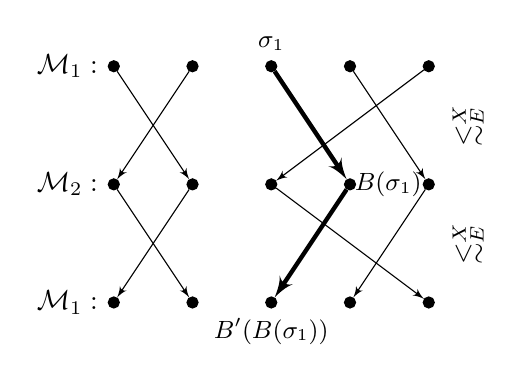
\begin{tikzpicture}
 \newcommand{\vLength}{1.5}
	\tikzset{vertex/.style = {circle,draw,fill=black,minimum size=4pt,inner sep=0pt}}
	\tikzstyle{edge} = [->,> = latex',thin]
	\tikzstyle{edgeThick} = [->,> = latex', ultra thick]
	%M_1
	\node[vertex] (00) at (0,\vLength) [label=left:$\mathcal{M}_1:$] {};
	\node[vertex] (01) at (1,\vLength) {};
	\node[vertex] (02) at (2,\vLength) [label=above:\small{$\sigma_1$}] {};
	\node[vertex] (03) at (3,\vLength) {};
	\node[vertex] (04) at (4,\vLength) {};
	%M_2
	\node[vertex] (10) at (0,0) [label=left:$\mathcal{M}_2:$] {};
	\node[vertex] (11) at (1,0) {};
	\node[vertex] (12) at (2,0) {};
	\node[vertex] (13) at (3,0) [label=right:\hspace{-4pt}\small{$B(\sigma_1)$}] {};
	\node[vertex] (14) at (4,0) {};
	%M_1 bottom
	\node[vertex] (20) at (0,-\vLength)[label=left:$\mathcal{M}_1:$] {};
	\node[vertex] (21) at (1,-\vLength) {};
	\node[vertex] (22) at (2,-\vLength) [label=below:\small{$B'(B(\sigma_1))$}] {};
	\node[vertex] (23) at (3,-\vLength) {};
	\node[vertex] (24) at (4,-\vLength) {};
	%mapping B
	\draw[edge] (00) to (11);
	\draw[edge] (01) to (10);
	\draw[edgeThick] (02) to (13);
	\draw[edge] (03) to (14);
	\draw[edge] (04) to (12);
	%mapping B'
	\draw[edge] (11) to (20);
	\draw[edge] (10) to (21);
	\draw[edgeThick] (13) to (22);
	\draw[edge] (14) to (23);
	\draw[edge] (12) to (24);
	
	\node[rotate=90] (B) at (4.5,0.5*\vLength) {$\moreGeneral$};
	\node[rotate=90] (B') at (4.5,-0.5*\vLength) {$\moreGeneral$};
\end{tikzpicture}
\end{center}
Since by definition $B'(B(\sigma_1))\moreGeneral B(\sigma_1)\moreGeneral\sigma_1$ $E$-minimality of $\mathcal{M}_1$ implies that $B'(B(\sigma_1))=\sigma_1$ for all $\sigma_1\in\mathcal{M}_1$. Symmetrically, $B(B'(\sigma_2))=\sigma_2$ for all $\sigma_2\in\mathcal{M}_2$.
\begin{center}
 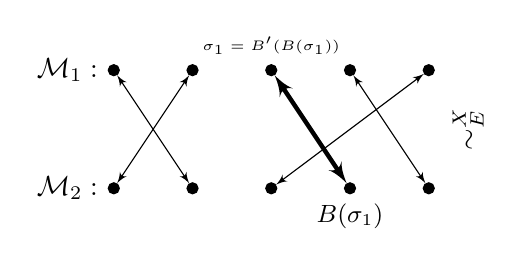
\begin{tikzpicture}
 \newcommand{\vLength}{1.5}
	\tikzset{vertex/.style = {circle,draw,fill=black,minimum size=4pt,inner sep=0pt}}
	\tikzstyle{edge} = [<->,> = latex',thin]
	\tikzstyle{edgeThick} = [<->,> = latex', ultra thick]
	%M_1
	\node[vertex] (00) at (0,\vLength) [label=left:$\mathcal{M}_1:$] {};
	\node[vertex] (01) at (1,\vLength) {};
	\node[vertex] (02) at (2,\vLength) [label=above:\tiny{$\sigma_1=B'(B(\sigma_1))$}] {};
	\node[vertex] (03) at (3,\vLength) {};
	\node[vertex] (04) at (4,\vLength) {};
	%M_2
	\node[vertex] (10) at (0,0) [label=left:$\mathcal{M}_2:$] {};
	\node[vertex] (11) at (1,0) {};
	\node[vertex] (12) at (2,0) {};
	\node[vertex] (13) at (3,0) [label=below:\small{$B(\sigma_1)$}] {};
	\node[vertex] (14) at (4,0) {};
	%mapping B
	\draw[edge] (00) to (11);
	\draw[edge] (01) to (10);
	\draw[edgeThick] (02) to (13);
	\draw[edge] (03) to (14);
	\draw[edge] (04) to (12);
	
	\node[rotate=90] (B) at (4.5,0.5*\vLength) {$\eqClass$};
\end{tikzpicture}
\end{center}
\end{proof}
	\section{Boolean Rings}
%intro
\[B:=\left\lbrace 
	\begin{aligned}
		x+y     & \approx y+x,         & x*y     & \approx y*x,     \\
		(x+y)+z & \approx x+(y+z),     & (x*y)*z & \approx x*(y*z), \\
		x+x     & \approx 0,           & x*x     & \approx x,       \\
		0+x     & \approx x,           & 0*x     & \approx 0,       \\
		x*(y+z) & \approx (x*y)+(x*z), & 1*x     & \approx x        
	\end{aligned}
	\right\rbrace \]
	Since $+$ and $*$ are associative we can omit most of the brackets. Furthermore we often write $xy$ instead of $x*y$.
	Lets consider an interpretation of $B$ the two element boolean ring $\BTwo$ with the carrier set $\textbf{2}:=\left\lbrace\bot,\top\right\rbrace$ where $*$ is \textquotedblleft and\textquotedblright\ and $+$ is \textquotedblleft exclusive or\textquotedblright:
	\begin{align*}
		(x+y)^\BTwo & :=\left( x^\BTwo\wedge\neg y^\BTwo\right)  \vee \left( \neg x^\BTwo\wedge y^\BTwo\right) & (x*y)^\BTwo & :=x^\BTwo\wedge y^\BTwo \\
		0^\BTwo     & :=\bot                                                                                      & 1^\BTwo     & :=\top                
	\end{align*}
	%TODO exercise 10.26
	It is easy to see that $\BTwo$ is indeed a model of $B$. Furthermore we can transform a term back from an Boolean algebra into Boolean ring theory:
	\begin{align*}
		x \wedge y & \mapsto x*y     \\
		x\vee y    & \mapsto x+y+x*y \\
		\neg x     & \mapsto x+1
	\end{align*}
	We work with + and * instead of $\vee,\wedge$ and $\neg$ because in Boolean rings we have a very convenient normal form which makes the following proofs easier.\\
	% maybe rephrase
	Lets consider another model of $B$ the powerset interpretation $\PSet$ with the carrier set $2^S$:
	\begin{align*}
		(x+y)^\PSet & :=x^\PSet\Delta y^\PSet & (x*y)^\PSet & :=x^\PSet\cap y^\PSet \\
		0^\PSet     & :=\emptyset             & 1^\PSet     & :=S                   
	\end{align*}
	Where $x\Delta y:=(x\setminus y)\cup(y\setminus x)$ is the symmetric difference of x and y. It is easy to see why $\PSet$ is a model of $B$. Lets just consider distributivity in detail.
	\begin{align*}
		\left( x*\left( y+z\right) \right) ^\PSet & =x^\PSet\cap\left( y^\PSet\Delta z^\PSet\right)                                                                                                                                                \\
		                                          & =x^\PSet\cap\left( \left( y^\PSet\setminus z^\PSet\right) \cup\left( z^\PSet\setminus y^\PSet\right) \right)                                                                                   \\
		                                          & =\left( \left( x^\PSet\cap y^\PSet\right) \setminus z^\PSet\right) \cup\left( \left( x^\PSet\cap z^\PSet\right) \setminus y^\PSet\right)                                                       \\
		                                          & =\left( \left( x^\PSet\cap y^\PSet\right) \setminus \left( x^\PSet\cap z^\PSet\right) \right) \cup\left( \left( x^\PSet\cap z^\PSet\right) \setminus \left( x^\PSet\cap y^\PSet\right) \right) \\
		                                          & =\left( x^\PSet\cap y^\PSet\right) \Delta \left( x^\PSet\cap z^\PSet\right)                                                                                                                    \\
		                                          & =\left( \left( x*y\right) +\left( x*z\right)\right)^\PSet                                                                                                                                      
	\end{align*}
	Here is a less formal explanation for why this identity holds in $\PSet$.\\
	\def\f{1.3}
	\def\CircleX{(\f*0.5,\f*0.866) circle (\f*0.8)}
	\def\CircleY{(\f*0,0) circle (\f*0.8)}
	\def\CircleZ{(\f*1,0) circle (\f*0.8)}
	\begin{tabular*}{\textwidth}{cc}
		\begin{tikzpicture}[fill=gray]
			\begin{scope}
				\clip \CircleY
				\CircleZ;
				\fill \CircleX;
			\end{scope}
			% left hand
			\begin{scope}
				\clip (-2,-1.5) rectangle (3,2.366)
				\CircleZ;
				\fill[pattern=north east lines] \CircleY;
			\end{scope}
			% right hand
			\begin{scope}
				\clip (-2,-1.5) rectangle (3,2.366)
				\CircleY;
				\fill[pattern=north east lines] \CircleZ;
			\end{scope}
			% fill y \cap z white
			\begin{scope}
				\clip \CircleY;
				\fill[white] \CircleZ;
			\end{scope}
			% draw circles
			\draw \CircleX  node [above] {$x^\PSet$}
			\CircleY  node [left] {$y^\PSet$}
			\CircleZ  node [right] {$z^\PSet$}
			(-2,-1.5) rectangle (3,2.366) (-2,2.366) node [below right] {$S$}
			(-2,-1.5) node [below right] {$(x*(y+z))^\PSet$};
		\end{tikzpicture}
		&
		\begin{tikzpicture}[fill=gray]
			\begin{scope}
				\clip \CircleY
				\CircleZ;
				\fill \CircleX;
			\end{scope}
			% fill y \cap z white
			\begin{scope}
				\clip \CircleY;
				\fill[white] \CircleZ;
			\end{scope}
			% fill z /cap x 
			\begin{scope}
				\clip \CircleX;
				\fill[pattern=north west lines] \CircleZ;
			\end{scope}
			% fill y /cap x 
			\begin{scope}
				\clip \CircleX;
				\fill[pattern=north east lines] \CircleY;
			\end{scope}
			% draw circles
			\draw \CircleX  node [above] {$x^\PSet$}
			\CircleY  node [left] {$y^\PSet$}
			\CircleZ  node [right] {$z^\PSet$}
			(-2,-1.5) rectangle (3,2.366) (-2,2.366) node [below right] {$S$}
			(-2,-1.5) node [below right] {$((x*y)+(x*z))^\PSet$};;
		\end{tikzpicture}
	\end{tabular*}
	This small example should just show that there are other models of $B$ with rather common interpretations of + and * apart from $\BTwo$. Note that if $|S|=1$ then $\PSet$ and $\BTwo$ are isomorphic.
	%correct word?
	%TODO we only consider terms over 0,1,+,*
	\subsection{Polynomials}
	\begin{definition}
		A product of distinct variables is a \textbf{monomial} (e.g.$\ xyz$). And a sum of distinct monomials is a \textbf{polynomial} (e.g.$\ x+xy+yz$).
	\end{definition}
	We compare monomials and polynomials modulo commutativity and associativity. So two monomials are distinct iff the sets of variables occurring in them are distinct and two polynomials are distinct iff the sets of their monomials are distinct.
	Here are some examples for clarification:
	\begin{align*}
		yxz & =zyx     & xy+yz & =zy+xy  \\
		yx  & \neq yxz & xy+yz & \neq xy 
	\end{align*}
	Note that we did not introduce a new symbol for equality of polynomials and just use the same as for syntactic equality since it will be clear from the context which one we mean. Now we can transform every term over $\left\lbrace 0,1,+,*\right\rbrace$ 
	%TODO right order?
	 into a (w.r.t. equality of polynomials) unique $\approx_B$-equivalent polynomial, its \textbf{polynomial form}. Since 1 is the neutral element of * we write 1 for the polynomial containing only the empty monomial correspondingly we identify 0 with the empty polynomial. Now the polynomial form can be computed recursively as follows:\\
	\begin{description}
		\item[$x,0,1:$] This is the base case, variables and the constants 0 and 1 are already polynomials.
		\item[$t_1+t_2:$] Let $p_1$ and $p_2$ be the polynomial forms of $t_1$ and $t_2$ the polynomial form of $t_1+t_2$ is obtained by removing all pairs of equivalent monomials from $p_1+p_2$. Since we have $\left\lbrace0+x\approx x,x+x\approx0\right\rbrace\in B$  this rule preserves $\approx_E$-equivalence.
		%explain 0?
		\item[$t_1*t_2:$]  Let $p_1=m_1+\dots+m_k$ and $p_2=n_1+\dots+n_l$ be the polynomial forms of $t_1$ and $t_2$. The polynomial form of $t_1*t_2$ is obtained by removing all pairs of equivalent monomials from $p_1*p_2$ which when multiplied out is the sum
		\begin{align*}
			m_1*n_1+\dots+m_1*n_l+\dots+m_k*n_1+\dots+m_k*n_l 
		\end{align*} 
		where the product of two monomials $m=x_1\dots x_r$ and $n=y_1\dots y_s$ is the monomial obtained by removing repeated occurrences of the same variable from $x_1\dots x_r y_1\dots y_s$. Since we have $\left\lbrace x*x\approx x\right\rbrace\in B$  this rule preserves $\approx_E$-equivalence. Note that if $t_1=1$ then we multiply every monomial in $p_2$ with the empty monomial which does not change anything so the result is as expected just $p_2$.
	\end{description}
	The polynomial form of $t$ is denoted by $t{\downarrow_P}$.
	%t=_B t|P
	%example
	\begin{theorem}\label{basicBR}
		The following statements are equivalent:
		\begin{enumerate}
			\item $\BTwo\models s\approx t,$
			\item $s{\downarrow_P}=t{\downarrow_P},$
			\item $s\approx_B t.$
		\end{enumerate}
	\end{theorem}
	%TODO lemma 4.2 somewhere here
	\begin{proof}\mbox{}
		\begin{description}
			\item[$1\Rightarrow 2$] asd
			\item[$2\Rightarrow 3$] asdf
			\item[$3\Rightarrow 1$] dth
		\end{description}
	\end{proof}
	Lets consider a bigger example $s:=(y+1)(x+y)+(y+1)x$, $t:=0$ and go through 1,2 and 3 from theorem \ref{basicBR}.
	\begin{enumerate}
			\item $\BTwo$ is a model of $s\approx t$.
			\begin{align*}
				s^\BTwo & =\left( \left( y+1\right)\left( x+y\right)+\left( y+1\right)x\right)^\BTwo       \\
				& =\left( s_1^\BTwo\wedge \neg s_2^\BTwo\right)\vee\left( \neg s_1^\BTwo\wedge s_2^\BTwo\right) \\
				&\hspace{8pt}\begin{aligned}
				s_1 & =\left( y+1\right)^\BTwo\wedge\left( x+y\right)^\BTwo & s_2 & =   \left( y+1\right)^\BTwo\wedge x^\BTwo \\
				    & =\neg y^\BTwo\wedge\left( x+y\right)^\BTwo            &     & = \neg y^\BTwo\wedge x^\BTwo              \\
				&=\neg y^\BTwo\wedge\left( \left( x^\BTwo\wedge\neg y^\BTwo\right)\vee\left( \neg x^\BTwo\wedge y^\BTwo\right)\right)\\
				& = x^\BTwo\wedge\neg y^\BTwo
				\end{aligned}\\
				s^\BTwo & =\left( \left( x^\BTwo\wedge\neg y^\BTwo\right)\wedge \neg \left( \neg y^\BTwo\wedge x^\BTwo\right)\right)\vee\left( \neg\left( x^\BTwo\wedge\neg y^\BTwo\right)\wedge \left( \neg y^\BTwo\wedge x^\BTwo\right)\right) \\
				& =\left( x^\BTwo\wedge\left( \neg y^\BTwo\wedge \left( y^\BTwo\vee\neg x^\BTwo\right)\right)\right)\vee\left( \left( \left( \neg x^\BTwo\vee y^\BTwo\right)\wedge \neg y^\BTwo\right)\wedge x^\BTwo\right)              \\
				& =\left( x^\BTwo\wedge\neg y^\BTwo\wedge \neg x^\BTwo\right)\vee\left( \neg x^\BTwo\wedge \neg y^\BTwo\wedge x^\BTwo\right)                                                                                             \\
				& =\bot\vee\bot\\
				& =t^\BTwo 
			\end{align*}
			\item The polynomial forms $s{\downarrow_P}$ and $t{\downarrow_P}$ are equal.
			\begin{align*}
				s & \approx_B (y+1)(x+y)+(y+1)x \\
				  & \approx_B yx+yy+x+y+yx+x    \\
				  & \approx_B yx+yx+y+y+x+x     \\
				  & \approx_B 0
			\end{align*}
			\begin{align*}
				s{\downarrow_P}=0=t{\downarrow_P}
			\end{align*}
			\item $s\approx_B t$ is a consequence of $B$.
			\begin{align*}
				s & \approx_B (y+1)(x+y)+(y+1)x \\
				  & \approx_B (y+1)(x+y+x)      \\
				  & \approx_B y+y               \\
				  & \approx_B 0                 \\
				  & \approx_B t                 
			\end{align*}
		\end{enumerate}
		A nice consequence from theorem \ref{basicBR} is that $\approx_B$ is decidable, because we could just compare the computable polynomial forms, or test semantic equality in $\BTwo$.
		\subsection{Unification}
		Note that until now we have not said anything about unification we just introduced the equational theory $B$, the semantic interpretation $\BTwo$ and showed some properties of the word problem in $\approx_B$.
		%TODO intro
		\begin{lemma}\mbox{}
		\begin{enumerate}
		\item Every solution of $s\approxq_B t$ in $\BTwo$ can be viewed as a $B$-unifier.
		\item If $s\approxq_B t$ has a $B$-unifier then $s\approxq t$ has a solution in $\BTwo$.
		\end{enumerate}
		\end{lemma}
		%TODO before or after proof? Note that we did not use iff because not every unifier can be viewed as a solution in $\BTwo$. example
		\begin{proof}\mbox{}
		\begin{itemize}
		\item[(1)]Let $\varphi:V\mapsto\textbf{2}$ be a solution of $s\approxq t$ in $\BTwo$ and $\widehat{\varphi}$ the homeomorphic extension of $\varphi$, i.e. $\widehat{\varphi}(s)=\widehat{\varphi}(t)$. From $\varphi$ we now can define a mapping $\phi:V\mapsto \TermSet$ to ground terms in the following way:
		\begin{align*}
		\phi(x):=\begin{cases}
		1 & \text{if }\varphi(x)=\top\\
		0 & \text{if }\varphi(x)=\bot
		\end{cases}
		\end{align*}
		for all $x\in V$. Lets denote the homeomorphic extension of $\phi$ by $\widehat{\phi}$. Let $\psi:\TermAlgebra\mapsto\BTwo$ be an arbitrary homomorphism since $\widehat{\phi}$ is a mapping to ground terms $\psi\widehat{\phi}=\widehat{\varphi}$. So the following
		\begin{align*}
		\psi\left( \widehat{\phi}(s)\right)=\widehat{\varphi}(s)=\widehat{\varphi}(t)=\psi\left( \widehat{\phi}(t)\right) 
		\end{align*}
		holds for all homomorphisms $\psi$ and hence $\BTwo\models\widehat{\phi}(s)\approx\widehat{\phi}(t)$. Theorem \ref{basicBR} yields $\widehat{\phi}(s)\approx_B\widehat{\phi}(t)$, i.e. the mapping $\phi$ (which we got directly from the solution $\varphi$), when viewed as a substitution, is a $B$-unifier.
		%TODO replace phi
		\item[(2)] Let $\sigma$ be a $B$-unifier of $s\approxq_B t$, i.e. $\sigma(s)\approx_B\sigma(t)$. Now theorem \ref{basicBR} yields $\BTwo\models\sigma(s)\approx\sigma(t)$ and hence $\psi\left(\sigma (s)\right)=\psi\left(\sigma (t)\right)$ for all homomorphisms $\psi:\TermAlgebra\mapsto\BTwo$. Hence $\psi\sigma:V\mapsto\textbf{2}$ is a solution in $\BTwo$.
		%TODO \psi\sigma ok? V->\TermSet=(?)\TermAlgebra->2
		\end{itemize}
		\end{proof}
		%TODO more text?
		%example
		Lets consider the B-unification problem $x+y+z\approxq z+1$ as small example for clarification.
		\begin{itemize}
		\item[(1)]The mapping 
		\begin{align*}
		\varphi(w):=\begin{cases}
		\bot& \text{if }w=x\\
		\top& \text{if }w\neq x
		\end{cases}
		\end{align*}is a solution of our problem. The substitution $\sigma:=\left\lbrace x\mapsto0,y\mapsto1,z\mapsto1\right\rbrace$ is $\varphi$ viewed as a $B$-unifier.
		\item[(2)]The substitution $\sigma':=\left\lbrace y\mapsto x+1,z\mapsto 1\right\rbrace $ obviously is a $B$-unifier. Let $\varphi$ be a mapping with $\varphi(x):=\top$ for all $x\in V$ and $\widehat{\varphi}$ its homeomorphic extension.
		\begin{align*}
		\widehat{\varphi}\left(\sigma'(w)\right)=\begin{cases}
		(\top+1)^\BTwo=\bot& \text{if } w=y\\
		1^\BTwo=\top& \text{if } w=z\\
		\top&  \text{otherwise}
		\end{cases}
		\end{align*}
		is a solution in $\BTwo$.
		\end{itemize}
		%TODO intro unitary,t\approx0
		\subsection{Successive variable elimination}
		The idea of this unification algorithm is %TODO intro
		
		Every term $t$ can be written as $x*r+(x+1)*s$ such that $x\notin\mathcal{V}ar(r,s)\subset\mathcal{V}ar(t)$. For example, we can split the polynomial form of $t$ into two sets of monomials, those who contain $x$  $\left(l_x\right)$ and those who do not contain $x$ $(s)$.Now $l$ is obtained by removing every occurrence of $x$ in $l_x$ and $r:=l+s$. To see why this works consider the small example $t:=yx+z$. Now $r:=y+z$ and $s:=z$.
		\begin{align*}
		x*(y+z)+(x+1)*z&\approx_B xy+xz+xz+z\\
		&\approx_B xy+z\\
		&\approx_B t
		\end{align*}
		This simple observation is the basis of successive variable elimination.
		Before we come to the main theorem of successive variable elimination we introduce a strong type of most general $B$-unifiers the reproductive $B$-unifiers.
		\begin{definition}
		A $E$-unifier $\sigma$ of a $B$-unification problem $S$ is a \textbf{reproductive $E$-unifier} iff $\tau(\sigma(x))\approx_E\tau(x)$ for every unifier $\tau$ of $S$ and every $x$.
		\end{definition}
		Note that for a normal mgu $\sigma$ of a $E$-unification problem $S$ it only has to hold that for every $E$-unifier $\tau$ of $S$ there has to exist a substitution $\theta$ such that $\theta(\sigma(x))\approx_E\tau(x)$ for every $x\in X$. 
		%TODO more explanation?
		\begin{theorem}
		Let $t\approx_B x*r+(x+1)*s$ such that $x\notin\mathcal{V}ar(r,s)\subset\mathcal{V}ar(t)$ and define $t':=r*s$.
		\begin{enumerate}
		\item Every $B$-unifier of $t\approxq_B0$ is a $B$-unifier of $t'\approxq_B0$.
		%reproductive unifier->mgu
		\item If $\sigma$ is a reproductive $B$-unifier of $t'\approxq_B0$ and $x\notin\mathcal{D}om(\sigma)$, then 
		\begin{align*}
		\sigma':=\sigma\cup\left\lbrace x\mapsto x*(\sigma(r)+\sigma(s)+1)+\sigma(s)\right\rbrace
		\end{align*}
		is a reproductive $B$-unifier of $t\approxq_B0$.
		\end{enumerate}
		\end{theorem}
		\begin{proof}\mbox{}
		\begin{itemize}
		\item[(1)] Let $\tau$ be a $B$-unifier of $t\approxq_B0$ and hence $\tau(t)\approx_B0$.
		\begin{align*}
		&&\tau(x)*\tau(r)+(\tau(x)+1)*\tau(s)&\approx_B0\\
		&\iff&\tau(x)*\tau(r)*\tau(s)+(\tau(x)+1)*\tau(s)*\tau(r)&\approx_B0*\tau(s)*\tau(r)\\
		&\iff&\tau(x)*\tau(r*s)+(\tau(x)+1)*\tau(s*r)&\approx_B0\\
		&\iff&(\tau(x)+\tau(x)+1)*\tau(s*r)&\approx_B0\\
		&\iff&\tau(s*r)&\approx_B0\\
		\end{align*}
		So $\tau$ is also a $B$-unifier of $t'\approxq_B0$.
		\item[(2)] Let $\sigma$ is a reproductive $B$-unifier of $t'\approxq_B0$ and $x\notin\mathcal{D}om(\sigma)$. It is easy to show that $\sigma'$ is a $B$-unifier of $t\approxq_B0$:
		\begin{align*}
		\sigma'(t)&\approx_B\sigma'(x)*\sigma'(r)+(\sigma'(x)+1)*\sigma'(s)\\
		&=\ \ (x*(\sigma(r)+\sigma(s)+1)+\sigma(s))*\sigma(r)+(\sigma'(x)+1)*\sigma(s)\\
		&\approx_B(x*(\sigma(r)+\sigma(s)*\sigma(r)+\sigma(r))+\sigma(s)*\sigma(r))+(\sigma'(x)+1)*\sigma(s)\\
		&\approx_B(x*(0+\sigma(s*r))+\sigma(s*r))+(\sigma'(x)+1)*\sigma(s)\\
		&\approx_B(x*\sigma(t')+\sigma(t'))+(\sigma'(x)+1)*\sigma(s)\\
		&\approx_B0+(x*(\sigma(r)+\sigma(s)+1)+\sigma(s)+1)*\sigma(s)\\
		&\approx_B(x*(\sigma(r)*\sigma(s)+\sigma(s)+\sigma(s))+\sigma(s)+\sigma(s))\\
		&\approx_B(x*(\sigma(r*s))+0)\\
		&\approx_B0\\
		\end{align*}
		Now we show that $\sigma'$ is also reproductive. Let $\tau$ be a $B$-unifier of $t\approxq_B0$. Because $\sigma$ is a reproductive $B$-unifier of $t'\approxq_B0$ and (1) implies that $\tau$ is indeed a $B$-unifier of $t'\approxq_B0$ it follows that $\tau(\sigma(y))\approx_B\tau(y)$ for all $y$. Therefore $\tau(\sigma'(y))=\tau(\sigma(y))\approx_B\tau(y)$ for all $y\neq x$. For $y=x$:
		\begin{align*}
		\tau(\sigma'(x))&=\ \ \tau(x*(\sigma(r)+\sigma(s)+1)+\sigma(s))\\
		&\approx_B \tau(x)*(\tau(\sigma(r))+\tau(\sigma(s))+1)+\tau(\sigma(s))\\
		&\approx_B \tau(x)*(\tau(r)+\tau(s)+1)+\tau(s)\\
		&\approx_B \tau(x)*\tau(r)+\tau(x)*\tau(s)+\tau(x)+\tau(s)\\
		&\approx_B \tau(x)*\tau(r)+(\tau(x)+1)*\tau(s)+\tau(x)\\
		&\approx_B \tau(t)+\tau(x)\\
		&\approx_B \tau(x)\\
		\end{align*}
		\end{itemize}
		\end{proof}
		%TODO outtro+example
		\subsection{Löwenheim's formula}
		This algorithm is not as intuitive as successive variable elimination but much more interesting. The idea is to turn an arbitrary $B$-unifier $\tau$ of $t\approxq_B0$ into an mgu (even a reproductive $B$-unifier).
		\begin{theorem}\label{lowenheim}
		Let $\tau$ be a $B$-unifier of $t\approxq_B0$. The substitution $\sigma$ defined by
		\begin{align*}
		\sigma(x):=\begin{cases}
		(t+1)*x+t*\tau(x) &\text{if }x\in\mathcal{V}ar(t) \\
		x &\text{if }x\notin\mathcal{V}ar(t)
		\end{cases}
		\end{align*}
		is a reproductive $B$-unifier of $t\approxq_B0$.
		\end{theorem}
		Before we can proof this theorem we need the following lemma to proof that $\sigma$ actually is a $B$-unifier. 
		\begin{lemma}
		If $\sigma(x)=(s+1)*\sigma_1(x)+s*\sigma_2(x)$ for all $x\in\mathcal{V}ar(t)$, then $\sigma(t)=(s+1)*\sigma_1(t)+s*\sigma_2(t)$.
		\end{lemma}
		\begin{proof}
		We show this by structural induction on $t$.
		\begin{itemize}
		\item[$t=x:$]The base case is trivial:
				\begin{align*}
				\sigma(t)&=(s+1)*\sigma_1(x)+s*\sigma_2(x)\\
				&=(s+1)*\sigma_1(t)+s*\sigma_2(t)
				\end{align*}
		\item[$t=0:$]
				\begin{align*}
				\sigma(t)&=0
				\approx_B0+0
				\approx_B(s+1)*0+s*0\\
				&=(s+1)*\sigma_1(t)+s*\sigma_2(t)
				\end{align*}
		\item[$t=1:$]
				\begin{align*}
				\sigma(t)&=1
				\approx_Bs+1+s
				\approx_B(s+1)*1+s*1\\
				&=(s+1)*\sigma_1(t)+s*\sigma_2(t)
				\end{align*}
		\item[$t=t_1+t_2:$]Using the induction hypothesis we obtain:
				\begin{align*}
				\sigma(t)&=\ \ \sigma(t_1)+\sigma(t_2)\\
				&\approx_B(s+1)*\sigma_1(t_1)+s*\sigma_2(t_1)+(s+1)*\sigma_1(t_2)+s*\sigma_2(t_2)\\
				&\approx_B(s+1)*(\sigma_1(t_1)+\sigma_1(t_2))+s*(\sigma_2(t_1)+\sigma_2(t_2))\\
				&=\ \ (s+1)*\sigma_1(t)+s*\sigma_2(t)\\
				\end{align*}
		\item[$t=t_1*t_2:$]Using the induction hypothesis we obtain:
				\begin{align*}
				\sigma(t)&=\ \ \sigma(t_1)*\sigma(t_2)\\
				&\approx_B((s+1)*\sigma_1(t_1)+s*\sigma_2(t_1))*((s+1)*\sigma_1(t_2)+s*\sigma_2(t_2))\\
				&\approx_B(s+1)*\sigma_1(t_1)*\sigma_1(t_2)+0+0+s*\sigma_2(t_1)*\sigma_2(t_2)\\
				&=\ \ (s+1)*\sigma_1(t)+s*\sigma_2(t)\\
				\end{align*}
		\end{itemize}
		\end{proof}
		Now we can proof theorem \ref{lowenheim}.
		\begin{proof}[Proof.(Theorem \ref{lowenheim})]
		
		\end{proof}
		%TODO in Löwenheims formular in example show that the different mgus are reproductive (in \eqClass)
\end{document}
